\documentclass[12pt]{report}
\usepackage[spanish]{babel}
\usepackage[utf8]{inputenc}
\usepackage{amsmath}
\usepackage{amssymb}
\usepackage{amsthm}
\usepackage{graphics}
\usepackage{subfigure}
\usepackage{lipsum}
\usepackage{array}
\usepackage{multicol}
\usepackage{enumerate}
\usepackage[framemethod=TikZ]{mdframed}
\usepackage[a4paper, margin = 1.5cm]{geometry}
\usepackage{tikz}
\usepackage{pgffor}
\usepackage{ifthen}
\usepackage{enumitem}
\usepackage{hyperref}
\usepackage{bbm}
\usepackage{listings}
\usetikzlibrary{graphs}

%Gestión de Hipervínculos

\hypersetup{
    colorlinks=true,
    linkcolor=black,
    filecolor=magenta,      
    urlcolor=cyan
}

%Gestión de Código de Programación

\definecolor{listing-background}{HTML}{F7F7F7}
\definecolor{listing-rule}{HTML}{B3B2B3}
\definecolor{listing-numbers}{HTML}{B3B2B3}
\definecolor{listing-text-color}{HTML}{000000}
\definecolor{listing-keyword}{HTML}{435489}
\definecolor{listing-keyword-2}{HTML}{1284CA} % additional keywords
\definecolor{listing-keyword-3}{HTML}{9137CB} % additional keywords
\definecolor{listing-identifier}{HTML}{435489}
\definecolor{listing-string}{HTML}{00999A}
\definecolor{listing-comment}{HTML}{8E8E8E}

\lstdefinestyle{myStyle}{
    language         = C++,
    alsolanguage     = scala,
    numbers          = left,
    xleftmargin      = 2.7em,
    framexleftmargin = 2.5em,
    backgroundcolor  = \color{gray!15},
    basicstyle       = \color{listing-text-color}\linespread{1.0}\ttfamily,
    breaklines       = true,
    frameshape       = {RYR}{Y}{Y}{RYR},
    rulecolor        = \color{black},
    tabsize          = 2,
    numberstyle      = \color{listing-numbers}\linespread{1.0}\small\ttfamily,
    aboveskip        = 1.0em,
    belowskip        = 0.1em,
    abovecaptionskip = 0em,
    belowcaptionskip = 1.0em,
    keywordstyle     = {\color{listing-keyword}\bfseries},
    keywordstyle     = {[2]\color{listing-keyword-2}\bfseries},
    keywordstyle     = {[3]\color{listing-keyword-3}\bfseries\itshape},
    sensitive        = true,
    identifierstyle  = \color{listing-identifier},
    commentstyle     = \color{listing-comment},
    stringstyle      = \color{listing-string},
    showstringspaces = false,
    label            = lst:bar,
    captionpos       = b,
}

\lstset{style = myStyle}

%Estilo del capítulo y sección

\makeatletter
\def\thickhrulefill{\leavevmode \leaders \hrule height 1ex \hfill \kern \z@}
\def\@makechapterhead#1{%
  {\parindent \z@ \raggedright
    \reset@font
    \hrule
    \vspace*{10\p@}%
    \par
    \center \LARGE \scshape \@chapapp{} \huge \thechapter
    \vspace*{10\p@}%
    \par\nobreak
    \vspace*{10\p@}%
    \par
    \vspace*{1\p@}%
    \hrule
    %\vskip 40\p@
    \vspace*{60\p@}
    \Huge #1\par\nobreak
    \vskip 50\p@
  }}

\def\section#1{%
  \par\bigskip\bigskip
  \hrule\par\nobreak\noindent
  \refstepcounter{section}%
  \addcontentsline{toc}{chapter}{#1}%
  \reset@font
  { \large \scshape
    \strut\S \thesection \quad
    #1}% 
    \hrule   
  \par
  \medskip
}

%Gestión marca de agua

\usetikzlibrary{shapes.multipart}

\newcounter{it}
\newcommand*\watermarktext[1]{\begin{tabular}{c}
    \setcounter{it}{1}%
    \whiledo{\theit<100}{%
    \foreach \col in {0,...,15}{#1\ \ } \\ \\ \\
    \stepcounter{it}%
    }
    \end{tabular}
    }

\AddToHook{shipout/foreground}{
    \begin{tikzpicture}[remember picture,overlay, every text node part/.style={align=center}]
        \node[rectangle,black,rotate=30,scale=2,opacity=0.04] at (current page.center) {\watermarktext{Cristo Daniel Alvarado ESFM\quad}};
  \end{tikzpicture}
}

%En esta parte se hacen redefiniciones de algunos comandos para que resulte agradable el verlos%

\def\proof{\paragraph{Demostración:\\}}
\def\endproof{\hfill$\blacksquare$}

\def\sol{\paragraph{Solución:\\}}
\def\endsol{\hfill$\square$}

%En esta parte se definen los comandos a usar dentro del documento para enlistar%

\newtheoremstyle{largebreak}
  {}% use the default space above
  {}% use the default space below
  {\normalfont}% body font
  {}% indent (0pt)
  {\bfseries}% header font
  {}% punctuation
  {\newline}% break after header
  {}% header spec

\theoremstyle{largebreak}

\newmdtheoremenv[
    leftmargin=0em,
    rightmargin=0em,
    innertopmargin=0pt,
    innerbottommargin=5pt,
    hidealllines = true,
    roundcorner = 5pt,
    backgroundcolor = gray!60!red!30
]{exa}{Ejemplo}[section]

\newmdtheoremenv[
    leftmargin=0em,
    rightmargin=0em,
    innertopmargin=0pt,
    innerbottommargin=5pt,
    hidealllines = true,
    roundcorner = 5pt,
    backgroundcolor = gray!50!blue!30
]{obs}{Observación}[section]

\newmdtheoremenv[
    leftmargin=0em,
    rightmargin=0em,
    innertopmargin=0pt,
    innerbottommargin=5pt,
    rightline = false,
    leftline = false
]{theor}{Teorema}[section]

\newmdtheoremenv[
    leftmargin=0em,
    rightmargin=0em,
    innertopmargin=0pt,
    innerbottommargin=5pt,
    rightline = false,
    leftline = false
]{propo}{Proposición}[section]

\newmdtheoremenv[
    leftmargin=0em,
    rightmargin=0em,
    innertopmargin=0pt,
    innerbottommargin=5pt,
    rightline = false,
    leftline = false
]{cor}{Corolario}[section]

\newmdtheoremenv[
    leftmargin=0em,
    rightmargin=0em,
    innertopmargin=0pt,
    innerbottommargin=5pt,
    rightline = false,
    leftline = false
]{lema}{Lema}[section]

\newmdtheoremenv[
    leftmargin=0em,
    rightmargin=0em,
    innertopmargin=0pt,
    innerbottommargin=5pt,
    roundcorner=5pt,
    backgroundcolor = gray!30,
    hidealllines = true
]{mydef}{Definición}[section]

\newmdtheoremenv[
    leftmargin=0em,
    rightmargin=0em,
    innertopmargin=0pt,
    innerbottommargin=5pt,
    roundcorner=5pt
]{excer}{Ejercicio}[section]

%En esta parte se colocan comandos que definen la forma en la que se van a escribir ciertas funciones%

\newcommand\abs[1]{\ensuremath{\left|#1\right|}}
\newcommand\divides{\ensuremath{\bigm|}}
\newcommand\cf[3]{\ensuremath{#1:#2\rightarrow#3}}
\newcommand\contradiction{\ensuremath{\#_c}}
\newcommand\natint[1]{\ensuremath{\left[\big|#1\big|\right]}}
\newcommand{\bbm}[1]{\ensuremath{\mathbbm{#1}}}
\newcounter{figcount}
\setcounter{figcount}{1}
\newcommand\Aut[1]{\ensuremath{\textup{Aut}\left(#1\right)}}
\newcommand{\Cay}[1]{\ensuremath{\textup{Cay}\left(#1\right)}}
\newcommand{\gen}[1]{\ensuremath{\langle#1\rangle}}

\begin{document}
    \setlength{\parskip}{5pt} % Añade 5 puntos de espacio entre párrafos
    \setlength{\parindent}{12pt} % Pone la sangría como me gusta
    \title{Notas Teoría Geométrica de Grupos
    
    10° Escuela Oaxaqueña de Matemáticas}
    \author{Cristo Daniel Alvarado}
    \maketitle

    \tableofcontents %Con este comando se genera el índice general del libro%

    \newpage

    \chapter{Teoría Geométrica de Grupos}

    \section{Introducción}

    En los capítulos anteriores hemos hablado sobre 

    \begin{mydef}
        Un grupo discreto $G$ es tal que está dotado de la topología discreta.
    \end{mydef}

    \section{Aplicaciones de espacios cubrientes}

    \begin{theor}
        Dado un espacio cubriente de $X$, $\cf{p}{\widetilde{X}}{X}$, se tiene que $\pi_1(X)\curvearrowright\widetilde{X}$ vía transformaciones de Deck.
    \end{theor}

    \begin{theor}
        Un grupo $G$ actúa de manera libre en un árbol si y sólo si $G$ es grupo libre.
    \end{theor}

    \begin{proof}
        $\Rightarrow):$ Supongamso que $G$ actúa de manera libre en un árbol $T$. Considere la función proyección $\cf{p}{T}{T/G}$. Afirmamos que $p$ es una función cubriente, en efecto...

        Se tien que $T/G$ es una gráfica, por lo cual:
        \begin{equation*}
            \pi_1(T/G)\cong F_n
        \end{equation*}
        para algún $n\in\mathbb{N}\cup\left\{\infty\right\}$. Usando transormaciones de Deck deducimos que:
        \begin{equation*}
            \pi_1(T/G)\cong G
        \end{equation*}
        por lo cual $G$ es libre.

        $\Leftarrow):$ Supongamos que $G$ es grupo libre, entonces existe un conjunto $S$ tal que $G=F(S)$. Notemos que:
        \begin{equation*}
            F(S)\cong\pi_1\left(X=\bigvee_{ s\in S}\bbm{S}^1 \right)
        \end{equation*}
        Se tiene que este espacio admite un cubrente universal, digamos $\cf{p}{\widetilde{X}}{X}$. Por un teorema, $\widetilde{X}$ es una gráfica y, por ser una gráfica tal que su grupo fundamental es trivial, entonces debe ser un árbol. También se probó que:
        \begin{equation*}
            \textup{Deck}(\widetilde{X})\rightarrow\widetilde{X}
        \end{equation*}
        actúa sobre este árbol (mediante $f\in\textup{Deck}(\widetilde{X})$).
    \end{proof}

    \begin{obs}
        Completar lo anterior formalmente y unir todo con las notas anteriores.
    \end{obs}

    \begin{propo}
        El grupo libre $F_2$ contiene como subgrupo de índice finito a $F_n$, para todo $n\geq2$.
    \end{propo}

    \begin{proof}
        
    \end{proof}

    La explicación de la proposición anterior es que, 

    \begin{excer}
        Encontrar un cubriente $\widetilde{X}$ de $X$ con $\pi_1(X)=F_2$ tal que $\pi_1(\widetilde{X})=F_1$.
    \end{excer}

    \section{Producto Semidirecto de Grupos}

    \begin{mydef}
        Sean $G$ y $H$ grupos, y sea $\cf{\varphi}{H}{\textup{Aut}(G)}$ un morfismo de grupos.

        Definimos el \textbf{producto semidirecto $G\rtimes_{\varphi} H$}, como el grupo en $G\times H$ con la operación dada por:
        \begin{equation*}
            (g_1,h_1)(g_2,h_2)=\left(g_1\varphi_{ h_1}(g_1^{-1}),h_1h_2 \right)
        \end{equation*}
    \end{mydef}

    \begin{propo}
        Probar que dados dos grupos $G$ y $H$, su producto semidirecto es un grupo.
    \end{propo}

    \begin{proof}
        Ejercicio.
    \end{proof}

    \begin{exa}
        Sean $G$ y $H$ grupos, y tomemos $\cf{\varphi}{G}{\textup{Aut}(H)}$ el homomorfismo trivial. Entonces:
        \begin{equation*}
            G\rtimes_{\varphi} H\cong G\times H
        \end{equation*} 
    \end{exa}

    \begin{exa}
        Si $K$ es la botella de Klein, entonces:
        \begin{equation*}
            \pi_1(K)\cong\bbm{Z}\rtimes\bbm{Z}
        \end{equation*}
    \end{exa}

    \begin{proof}
        Recordemos que:
        \begin{equation*}
            \pi_1(K)\cong\langle a,b|aba=b^{-1}\rangle
        \end{equation*}
        y, observemos que todo homomorfismo $\cf{f}{\bbm{Z}}{\textup{Aut}(\bbm{Z})}$ solo tiene de dos:
        \begin{equation*}
            \varphi(1)=\pm\bbm{1}_{\bbm{Z}}
        \end{equation*}
        completar la demostración.
    \end{proof}

    \begin{excer}
        Pruebe que $D_\infty\cong\bbm{Z}\rtimes\bbm{Z}_2$.
    \end{excer}

    \begin{proof}
        Recordemos que:
        \begin{equation*}
            D_\infty=\textup{Aut}(\bbm{R})
        \end{equation*}
        tomando los automorfismos de $\bbm{R}$ como gráfica (con nodos los enteros $\bbm{Z}$).
    \end{proof}

    \section{Grupos finitamente generados y Gráfica de Caley}

    \begin{mydef}
        Un grupo $G$ se dice \textbf{finitamente generado} si existe un conjunto $S\subseteq G$ finito tal que $G=\langle S\rangle$.
    \end{mydef}

    \begin{exa}
        $\bbm{Z}=\langle1\rangle$ es finitamente generado.
    \end{exa}

    \begin{mydef}
        Sea $G$ un grupo finitamente generado, y sea $S\subseteq G$ un conjunto finito de generadores de $G$. La \textbf{gráfica de Caley}, denotada por $\textup{Cay}(G,S)$ se define como una gráfica en la que:
        \begin{itemize}
            \item Los vértices son elementos de $G$, es decir, $V(\textup{Cay}(G,S))=G$.
            \item Las aristas se construyen de la siguiente manera: para cada vértice $g\in G$ y cada $s\in S\cup S^{-1}\setminus\left\{1\right\}$, se dibuja una arista entre $g$ y $gs$.
        \end{itemize}
    \end{mydef}

    \begin{exa}
        Considere $G=\bbm{Z}$ y $S=\left\{1\right\}$. Entonces, la gráfica de Caley estará dada por la gráfica de $\bbm{R}$ con $\bbm{Z}$ los vértices de la gráfica.
    \end{exa}

    \begin{exa}
        Considere $G=\bbm{Z}$ y $S=\left\{2,3\right\}$ ¿cuál es la gráfica de Caley?
    \end{exa}

    \begin{sol}
        Resulta que:
        
        \begin{minipage}{\textwidth}
            \begin{center}
                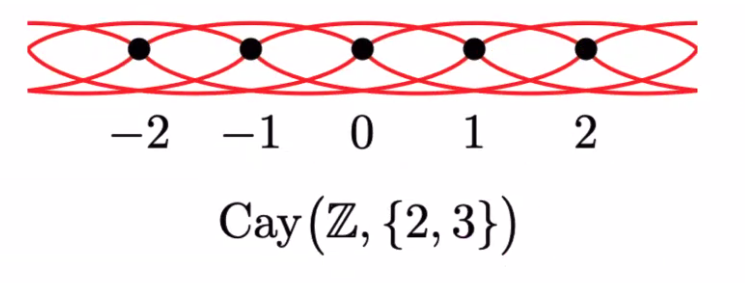
\includegraphics[scale=0.3]{images/Caley_2_3.png}\\
                Figura \thefigcount. Caption.
                \stepcounter{figcount}
            \end{center}
        \end{minipage}

        es la gráfica de Caley de esta cosa, que es diferente de la gráfica del ejemplo anterior. 
    \end{sol}

    \begin{propo}
        La gráfica de Caley $\textup{Caley}(G,S)$, para un grupo generado $G$ y un conjunto generador $S$, tiene las siguientes propiedades:
        \begin{itemize}
            \item Es arco-conexa (o conexa).
            \item Es localmente finita, es decir que cada vértice tiene solamente un conjunto finito de puntos como vecinos.
        \end{itemize}
    \end{propo}

    \section{Gráfica de Caley como espacio métrico}

    \begin{mydef}
        Dado un grupo $G$ finitamente generado por un conjunto $S$, definimos la \textbf{métrica de palabras} $d_S(g,h)$ entre dos elementos $g,h\in G$ como la longitud mínima de una palabra en los generadores $S\cup S^{-1}$ que representa a $g^{-1}h$.
    \end{mydef}

    \begin{obs}
        De ahora en adelante consideraremos a $\bbm{R}^n$ con la métrica euclideana.
    \end{obs}

    \begin{mydef}
        Sean $X$ y $Y$ espacios métricos. Una función $\cf{f}{X}{Y}$ se dice que es un encaje \textbf{isométrico} si:
        \begin{equation*}
            d(x,y)=\rho(f(x),f(y)),\quad\forall x,y\in X
        \end{equation*}
    \end{mydef}

    \begin{mydef}
        Sean $X$ y $Y$ espacios métricos. Una función $\cf{f}{X}{Y}$ se dice que es un \textbf{encaje bilipschitz} si existe $L\in\bbm{R}_{\geq0}$ tal que:
        \begin{equation*}
            \frac{1}{L}d_X(x,y)\leq d_Y(f(x),f(y))\leq Ld_X(x,y)
        \end{equation*}

        Decimos que $f$ es una \textbf{equivalencia bilipschitz} si existe una función $\cf{g}{Y}{X}$ encaje bilipschitz tal que:
        \begin{equation*}
            g\circ f=\bbm{1}_X\quad\textup{y}\quad f\circ g=\bbm{1}_Y
        \end{equation*}
    \end{mydef}

    \begin{mydef}
        Sea $\cf{f}{X}{Y}$ una función. Decimos que $f$ es un \textbf{encaje quasi-isométrico} si:
        \begin{equation*}
            \frac{1}{c}d_X(x,y)-b\leq d_Y(f(x),f(y))\leq cd_X(x,y)+b
        \end{equation*}
        con $c\geq1$ y $d\geq0$.
    \end{mydef}

    \newcommand{\floor}[1]{\ensuremath{\lfloor #1\rfloor}}

    \begin{exa}
        Consideremos a $\bbm{R}$ con la métrica euclideana y tomemos el encaje $\cf{i}{\bbm{Z}}{\bbm{R}}$. Queremos encontrar constates $c\geq1$ y $b\geq0$ tales que:
        \begin{equation*}
            \frac{1}{c}\abs{n-m}-b\leq\abs{i(n)-i(m)}\leq c\abs{n-m}+b
        \end{equation*}
        para todo $n,m\in\bbm{Z}$. Podemos elegir $b=0$ y $c=1$, con lo cual sucede que:
        \begin{equation*}
            \abs{n-m}\leq\abs{i(n)-i(m)}\leq \abs{n-m}
        \end{equation*}
        para todo $n,m\in\bbm{Z}$.
    \end{exa}

    \begin{exa}
        Consideremos la función parte entera $x\mapsto \floor{x}=\max\left\{n\in\mathbb{Z}\Big|n\leq x \right\}$. Afirmamos que $\floor{\cdot}$ es un encaje quasi-isométrico.
    \end{exa}

    \begin{proof}
        En efecto, sean $x,y\in\bbm{R}$, debemos encontrar $c\geq1$ y $b\geq0$ tales que:
        \begin{equation*}
            \frac{1}{c}\abs{x-y}-b\leq\abs{\floor{x}-\floor{y}}\leq c\abs{x-y}+b
        \end{equation*}
        Tomemos $c=b=1$. En efecto, sean $x,y\in\bbm{R}$, se tiene que:
        \begin{equation*}
            \abs{x-y}\leq \abs{\floor{x}-\floor{y}}+1
        \end{equation*}
        y, de forma análoga:
        \begin{equation*}
            \abs{\floor{x}-\floor{y}}\leq\abs{x-y}+1
        \end{equation*}
        con lo que se tienen las desigualdades deseadas.
    \end{proof}

    \newcommand{\qisom}{\ensuremath{\underset{C.I.}{\sim}}}

    \begin{mydef}
        Sea $\cf{f}{X}{Y}$ un $(c,b)$-encaje quasi-isométrico.
        \begin{enumerate}[label = \textit{(\alph*)}]
            \item Decimos que una función $\cf{f'}{X}{Y}$ está a \textbf{distancia fintia de $f$} si existe una constante $k\in\bbm{R}_{\geq0}$ tal que:
            \begin{equation*}
                d_Y(f(x),f'(x))\leq k,\quad\forall x\in X
            \end{equation*}
            \item Decimos que $f$ es una \textbf{quasi-isometría} si existe un encaje quasi-isométrico $\cf{g}{Y}{X}$ tal que $f\circ g$ está a distancia finita de $\bbm{1}_Y$ y $g\circ f$ lo está de $\bbm{1}_X$.
            \item Si $X$ es quasi-isométrico a $Y$, escribimos $X\qisom Y$.
        \end{enumerate}
    \end{mydef}

    \begin{mydef}
        Sea $\cf{f}{X}{Y}$. Decimos que $f$ tiene una \textbf{imagen quasi-densa} si existe $k\in\bbm{R}_{\geq0}$ tal que:
        \begin{equation*}
            \forall y\in Y \exists x\in X d_Y(y,f(x))\leq k
        \end{equation*}
    \end{mydef}

    \begin{theor}[\textbf{Caracterización de Quasi-isometrías}]
        Una función $\cf{f}{X}{Y}$ es una quasi-isometría si y sólo si $f$ es un encaje isométrico con imagen quasi-densa.
    \end{theor}

    \newcommand{\im}[1]{\ensuremath{\textup{im}\left(#1\right)}}

    \begin{proof}
        $\Rightarrow):$ Supongamos que $\cf{f}{X}{Y}$ es un encaje C.I. Veamos que $f$ es encaje quasi-isométrico y que $\im{f}\subseteq Y$ es quasi-densa.

        Claramente es encaje quasi-isométrico. Ahorra, por ser encaje C.I. existe una función $\cf{g}{Y}{X}$ encaje quasi-isométrico tal que:
        \begin{equation*}
            d_Y(f\circ g,\bbm{1}_Y)\leq k
        \end{equation*}
        para aklgún $k\in\bbm{R}_{\geq0}$. Entonces, si $y\in Y$ existe $x=g(y)\in X$ tal que:
        \begin{equation*}
            d_Y(f(x),y)\leq k
        \end{equation*}
        por lo que la imagen de $f$ es quasi-densa.

        $\Leftarrow):$ Supongamos que $\cf{f}{X}{Y}$ es un $(c,b)$ encaje quasi-isométrico con imagen quasi-densa, es decir que:
        \begin{equation*}
            \frac{1}{c}d_X(x,y)-b\leq d_Y(f(x),f(y))\leq cd_X(x,y)+b
        \end{equation*}
        $\forall x,y\in X$. Y además, existe $c^*\in\bbm{R}_{\geq0}$ tal que $\forall y\in Y$ existe $x\in X$ tal que:
        \begin{equation*}
            d_Y(f(x),y)\leq c^*
        \end{equation*}
        Tomemos $k=\max\left\{c,c^*,b \right\}\geq 1$. Entonces:
        \begin{equation*}
            \frac{1}{k}d_X(x,y)-k\leq d_Y(f(x),f(y))\leq kd_X(x,y)+k
        \end{equation*}
        y,
        \begin{equation*}
            d_Y(f(x),y)\leq k
        \end{equation*}

        Sea $y\in Y$, tomemos un $x_y\in X$ tal que:
        \begin{equation*}
            d_Y(f(x_y),y)\leq k
        \end{equation*}
        hagamos $g(y)=x_y$ para todo $y\in Y$.
    \end{proof}

    \begin{exa}
        Todo espacio métrico $X$ de diámetro finito es quasi-isométrico al espacio de un punto.
    \end{exa}

    \begin{mydef}
        Sea $G$ un grupo actuando en una gráfica $(V,E)$, esto es, tenemos un homomorfismo $\cf{\varphi}{G}{\Aut{V,E}}$. La acción $\varphi$ es \textbf{libre} si para todo $g\in G\setminus\left\{e\right\}$:
        \begin{equation*}
            \forall v\in V, \varphi_g(v)\neq v
        \end{equation*}
        y,
        \begin{equation*}
            \forall\left\{v,w \right\}\in E,\varphi_g\left(\left\{v,w \right\}\right) \left\{\varphi_g(v),\varphi_g(w) \right\}\neq \left\{v,w \right\}
        \end{equation*}
    \end{mydef}

    \begin{exa}
        Suponga que $G=\gen{S}$, entonces tenemos una acción:
        \begin{equation*}
            \cf{\varphi}{G}{\Aut{V,E}}
        \end{equation*}
        tal que $g\mapsto g\cdot h$.
    \end{exa}

    \begin{obs}
        La acción se reestringe a:
        \begin{equation*}
            \cf{\varphi}{G}{\Aut{G}}
        \end{equation*}
        tal que $g\mapsto\varphi_g$. Afirmamos que esta acción es libre.
    \end{obs}

    \begin{proof}
        En efecto, se tiene que:
        \begin{equation*}
            \begin{split}
                \varphi_g(h)=h&\iff g\cdot h=h\\
                &\iff g=e\\
            \end{split}
        \end{equation*}
        así que la acción es libre.
    \end{proof}

    \begin{mydef}
        Una acción $G\curvearrowright X$ es \textbf{transitiva} si $\forall x\in X$ tenemos que:
        \begin{equation*}
            \mathcal{O}_x=\left\{gx\Big|g\in X \right\}=X
        \end{equation*}
    \end{mydef}

    \begin{propo}
        Sea $G$ un grupo y $S\subseteq G$ un conjunto generador de $G$. Entonces, la acción $\cf{\varphi}{G}{\Aut{\Cay{G,S}}}$ dada por:
        \begin{equation*}
            g\mapsto(h\mapsto g\cdot h)
        \end{equation*}
        es libre si y sólo si no contiene involuciones, es decir que no existe $s\in S$ tal que $s^2=e$.
    \end{propo}

    \begin{proof}
        Sabemos que la acción $\varphi$ se reestringe a $G$ y es libre.

        $\Rightarrow):$ Supo

        $\Leftarrow):$ Supongamos que $\varphi$ no es libre, entonces existe una arista $\left\{v,w \right\}$ tal que:
        \begin{equation*}
            g\cdot\left\{v,w \right\}=\left\{v,w \right\}
        \end{equation*}
        para algún $g\in G\setminus\left\{e \right\}$. Tenemos dos casos:
        \begin{itemize}
            \item $g\cdot v=v$\contradiction, cosa que no puede suceder ya que la acción es libre sobre $G$.
            \item $g\cdot v=w$, por lo que $g\cdot w=v$, así que:
            \begin{equation*}
                v=g\cdot w=g(g\cdot v)=g^2\cdot v\Rightarrow g^2=e
            \end{equation*}
        \end{itemize}
        con lo que se sigue que $G$ tiene involuciones.
    \end{proof}

    \begin{propo}
        Sea $G$ un grupo finitamente generado. Entonces, la gráfica de Caley es única hasta quasi-isometrías.
    \end{propo}

    \begin{proof}
        Sean $S$ y $S'$ conjuntos finitos generadores de $G$. Probaremos que:
        \begin{equation*}
            \cf{\bbm{1}}{\Cay{G,S}}{\Cay{G,S'}}
        \end{equation*}
        es una equivalencia bilipschitz. Sea:
        \begin{equation*}
            n=\max\left\{d(e,s)\Big|s\in S' \right\}
        \end{equation*}
        Notemos que $n$ existe ya que el conjunto de la derecha es finito.
    \end{proof}

    \begin{mydef}
        Dos grupos $G$ y $H$ son \textbf{quasi-isométricos} si $\Cay{G,S}\qisom\Cay{H,T}$.
    \end{mydef}

    \begin{exa}
        Todos los grupos finitos son quasi-isométricos.
    \end{exa}

    ¿Cómo clasificar grupos hasta quasi-isometrías?

    La primera respuesta es construír invariantes quasi-isométricos.

    \chapter{Ejercicios y Problemas}

    \section{Introducción a la teoría geométrica de grupos}
    
    \begin{excer}
        Utilizando la teoría de cubrientes demuestra que:
        \begin{enumerate}[label = \textit{(\arabic*)}]
            \item Todo subgrupo de índice finito en un grupo finitamente generado es finitamente generado.
            \item Todo subgrupo de índice finito en un grupo finitamente presentado es finitamente presentado.
        \end{enumerate}
    \end{excer}

    \begin{proof}
        De \textit{(1)}: Sea $G$ un grupo finitamente generado y $H<G$ tal que $[G:H]<\infty$.


    \end{proof}

    \begin{excer}
        Demuestra que en el producto semidirecto $N\rtimes_{\varphi}H$, $H$ es un subgrupo normal si y sólo si $\varphi$ es el homomorfismo trivial.
    \end{excer}

    \begin{proof}
        Recordemos que el producto semidirecto $N\rtimes_\varphi H$ es el grupo $N\times H$ dotado de la operación:
        \begin{equation*}
            (n,h)(n',h')=(n\varphi_h(n'),hh')
        \end{equation*}
        donde $\cf{\varphi}{H}{\Aut{N}}$ es un homomorfismo tal que $h\mapsto\varphi_h$. El elemento neutro de este grupo es $(e_N,e_H)$, donde cada elemento tiene como inverso:
        \begin{equation*}
            (n,h)^{-1}=\left((\varphi_{h^{-1}}(n))^{-1},h^{-1}\right)
        \end{equation*}

        Sean $(n_1,h_1)\in N\rtimes_{\varphi}H$ y $h\in H$, se tiene que:
        \begin{equation*}
            \begin{split}
                (n_1,h_1)(e_N,h)(n_1,h_1)^{-1}&=(n_1,h_1)(e_N,h)\left((\varphi_{h_1^{-1}}(n_1))^{-1},h_1^{-1}\right)\\
                &=(n_1\varphi_{h_1}(e_N),h_1h)\left((\varphi_{h_1^{-1}}(n_1))^{-1},h_1^{-1}\right)\\
                &=(n_1\varphi_{h_1}(e_N),h_1h)\left((\varphi_{h_1^{-1}}(n_1))^{-1},h_1^{-1}\right)\\
                &=(n_1e_N,h_1h)\left((\varphi_{h_1^{-1}}(n_1))^{-1},h_1^{-1}\right)\\
                &=(n_1,h_1h)\left((\varphi_{h_1^{-1}}(n_1))^{-1},h_1^{-1}\right)\\
                &=\left(n_1\varphi_{h_1h}\left((\varphi_{h_1^{-1}}(n_1))^{-1}\right),h_1hh_1^{-1} \right)\\
                &=\left(n_1\varphi_{h_1h}\left((\varphi_{h_1^{-1}}(n_1^{-1}))\right),h_1hh_1^{-1} \right)\\
                &=\left(n_1\varphi_{h_1h h_1^{-1}}\left(n_1^{-1}\right),h_1hh_1^{-1} \right)\\
            \end{split}
        \end{equation*}
        pues, $\varphi_{h_1}(e_N)=e_N$ y por ser $h\mapsto\varphi_h$ homomorfismo.

        $\Rightarrow)$: Suponga que $H$ es un subgrupo normal de $N\rtimes_\varphi H$, esto es que el grupo $H$ visto como subgrupo de $N\rtimes_\varphi H$:
        \begin{equation*}
            H=\left\{(e_N,h)\Big|h\in H \right\}
        \end{equation*}
        es subgrupo normal de $N\rtimes_\varphi H$. Como es normal, se sigue que:
        \begin{equation*}
            (n_1,h_1)(e_N,h)(n_1,h_1)^{-1}\in H
        \end{equation*}
        para todo $(n_1,h_1)\in N\rtimes_{\varphi}H$ y $h\in H$, por lo que:
        \begin{equation*}
            \left(n_1\varphi_{h_1h h_1^{-1}}\left(n_1^{-1}\right),h_1hh_1^{-1} \right)\in H
        \end{equation*}
        nuevamente, para todo $(n_1,h_1)\in N\rtimes_{\varphi}H$ y $h\in H$. En particular:
        \begin{equation*}
            n_1\varphi_{h_1h h_1^{-1}}\left(n_1^{-1}\right)=e_N
        \end{equation*}
        por lo que para todo $n\in N$ y $h\in H$:
        \begin{equation*}
            n^{-1}\varphi_{h}\left(n\right)=e_N\Rightarrow\varphi_h(n)=n
        \end{equation*}
        es decir, que $\varphi_h=\bbm{1}_H$, por lo que $h\mapsto \varphi_h$ es el homomorfismo trivial.
        
        $\Leftarrow):$ Suponga que $\varphi$ es trivial, se sigue que:
        \begin{equation*}
            \begin{split}
                (n_1,h_1)(e_N,h)(n_1,h_1)^{-1}&=\left(n_1\varphi_{h_1h h_1^{-1}}\left(n_1^{-1}\right),h_1hh_1^{-1} \right)\\
                &=(n_1\bbm{1}_H(n_1^{-1}),h_1hh_1^{-1})\\
                &=(n_1n_1^{-1},h_1hh_1^{-1})\\
                &=(e_N,h_1hh_1^{-1})\in H\\
            \end{split}
        \end{equation*}
        para todo $(n_1,h_1)\in N\rtimes_{\varphi}H$ y $h\in H$, por lo que $H$ es normal en $N\rtimes_{\varphi}H$.
    \end{proof}

    \begin{excer}
        Demuestra que el grupo diédrico infinito $D_\infty$ es isomorfo tanto al producto libre $\bbm{Z}/2\bbm{Z}*\bbm{Z}/2\bbm{Z}$ como al producto semidirecto $\bbm{Z}\rtimes\bbm{Z}/2\bbm{Z}$.
    \end{excer}

    \begin{proof}
        Recordemos que:
        \begin{equation*}
            D_\infty=\gen{r,s\Big|s^2=1,srs=r^{-1}}
        \end{equation*}
        Probaremos que es isomorfo a ambos grupos.
        \begin{itemize}
            \item Observemos que el producto semidirecto $\bbm{Z}\rtimes\bbm{Z}/2\bbm{Z}$ es tal que el homomorfismo $\cf{\varphi}{\bbm{Z}/2\bbm{Z}}{\Aut{\bbm{Z}}}$ tiene dos opciones, o es el trivial, ya que:
            \begin{equation*}
                \varphi(0)=\bbm{1}_{\bbm{Z}}
            \end{equation*}
            y $\varphi(1)=-\bbm{1}_\bbm{Z}$, o:
            \begin{equation*}
                \varphi(x)=\bbm{1}_{\bbm{Z}},\quad\forall x\in\bbm{Z}/2\bbm{Z}
            \end{equation*}
            Analicemos ambos casos:
            \begin{itemize}
                \item Si $\varphi$ no es trivial, se sigue que:
                \begin{equation*}
                    \begin{split}
                        (x_1,y_1)(x_2,y_2)&=(x_1+\varphi_{ y_1}(x_2),y_1+y_2)\\
                        &=\left\{
                            \begin{array}{lcr}
                                (x_1+\bbm{1}_\bbm{Z}(x_2),0+y_2) & \textup{ si } & y_1=0 \\
                                (x_1-\bbm{1}_\bbm{Z}(x_2),1+y_2) & \textup{ si } & y_1=1 \\
                            \end{array}
                        \right.\\
                        &=\left\{
                            \begin{array}{lcr}
                                (x_1+x_2,y_2) & \textup{ si } & y_1=0 \\
                                (x_1-x_2,1+y_2) & \textup{ si } & y_1=1 \\
                            \end{array}
                        \right.\\
                    \end{split}
                \end{equation*}
                Afirmamos que en este caso, $D_\infty\cong\bbm{Z}\rtimes\bbm{Z}/2\bbm{Z}$. En efecto, considere la función $\cf{f}{D_\infty}{\bbm{Z}\rtimes\bbm{Z}/2\bbm{Z}}$ dada por:
                \begin{equation*}
                    f(r)=(1,0)\quad\textup{y}\quad f(s)=(0,1)
                \end{equation*}
                Como $D_\infty$ admite una presentación, $f$ se puede extender a un homomorfismo. Veamos que este homomorfismo es inyectivo y suprayectivo.
                \begin{itemize}
                    \item \textbf{$f$ es inyectiva}: Sea $s^{\epsilon_1}r^ns^{\epsilon_2}\in D_\infty$ con $\epsilon_1,\epsilon_2\in\left\{0,1\right\}$ y $n\in\mathbb{N}\cup\left\{0\right\}$ tal que:
                    \begin{equation*}
                        f(s^{\epsilon_1}r^ns^{\epsilon_2})=0
                    \end{equation*}
                    entonces:
                    \begin{equation*}
                        \begin{split}
                            f(s^{\epsilon_1}r^ns^{\epsilon_2})&=(0,\epsilon_1)(n,0)(0,\epsilon_2)\\
                            &=(0,\epsilon_1)(n,\epsilon_2)\\
                            &=\left\{
                                \begin{array}{lcr}
                                    (n, \epsilon_2) & \textup{ si } & \epsilon_1=0 \\
                                    (-n, 1+\epsilon_2) & \textup{ si } & \epsilon_1=1 \\
                                \end{array}
                            \right.\\
                        \end{split}
                    \end{equation*}
                    en cualquier caso, debe tenrse que $n=0$, por lo cual $\epsilon_2=0$ si $\epsilon_1=0$ y $\epsilon_2=1=\epsilon_1$, en cualquier caso se sigue que:
                    \begin{equation*}
                        s^{\epsilon_1}r^ns^{\epsilon_2}=1
                    \end{equation*}
                    por lo que $\ker(f)=\gen{1}$.
                    \item \textbf{$f$ es suprayectiva}: Sea $(m,\epsilon)\in\bbm{Z}\rtimes\bbm{Z}/2\bbm{Z}$. Veamos que:
                    \begin{equation*}
                        \begin{split}
                            f(r^ms^{\epsilon})&=(m,\epsilon)
                        \end{split}
                    \end{equation*}
                    es el elemento deseado.
                \end{itemize}
                Por ambos incisos se sigue que $f$ es isomorfismo.
            \end{itemize}
            \item Veamos que el producto libre $\bbm{Z}/2\bbm{Z}*\bbm{Z}/2\bbm{Z}$ está dado por:
            \begin{equation*}
                \bbm{Z}/2\bbm{Z}*\bbm{Z}/2\bbm{Z}=\gen{x,y\Big|x^2=1\textup{ y }y^2=1}
            \end{equation*}
            pues, $\bbm{Z}/2\bbm{Z}=\gen{x\Big|x^2=1}$. Los elementos de este grupo son sucesiones alternantes $xyxy\cdots$ o $yxyx\cdots$ de los elementos $x$ y $y$. Considere la función $\cf{f}{\bbm{Z}/2\bbm{Z}*\bbm{Z}/2\bbm{Z}}{D_\infty}$ dada por:
            \begin{equation*}
                f(x)=r\quad\textup{y}\quad f(y)=s
            \end{equation*}
            esta es función y más aún, puede ser extendida a un homeomorfismo ya que como el producto libre admite presentación basta con definirlo sobre los elementos de la base (usando además las propiedades de grupos libres).

            Por ende, veamos que es inyectiva y sobreyectiva:
            \begin{itemize}
                \item \textbf{$f$ es inyectiva}: Sea $z\in\bbm{Z}/2\bbm{Z}*\bbm{Z}/2\bbm{Z}$ tal que $f(z)=0$. Se tienen cuatro casos:
                \begin{enumerate}[label = \textit{(\alph*)}]
                    \item $z=xy\cdots xy$ sea $m$ el número de veces que aparece $r$ en este producto. Se sigue que $f(z)=f(x)f(y)\cdots f(x)f(y)=rs\cdots rs$. En esencia, todos los elementos están alternando y, usando el hecho de que en $D_\infty$ se cumple:
                    \begin{equation*}
                        rs=sr^{-1}
                    \end{equation*}
                    podemos reducir todo lo anterior a algo de la forma $s^{\epsilon}(r^{-1})^n$ con $\epsilon\in\left\{0,1\right\}$ y $n\in\mathbb{N}$. Se sigue así que:
                    \begin{equation*}
                        \begin{split}
                            f(z)=s^{\epsilon}r^n=0
                        \end{split}
                    \end{equation*}
                    y eso es cero si y sólo si $\epsilon=0$ y $n=0$. Pero $n$ está dado por el número de veces que cambiamos $r$ a la derecha, que fueron $m$-veces, es decir que $m=n$. Así que $m=0$. Por tanto, $z=0$.
                    \item Los otros casos son $z=xy\cdots yx$, $z=yx\cdots yx$ y $z=yx\cdots xy$, donde se procede de forma análoga al ejemplo anterior.
                \end{enumerate}
                \textbf{$f$ es sobreyectiva}. Sea $u\in D_\infty$. Por las propiedades de este grupo este elemento se expresa como:
                \begin{equation*}
                    s^{\epsilon_1} r^ns^{\epsilon_2}
                \end{equation*}
                donde $\epsilon_1,\epsilon_2\in\left\{0,1\right\}$ y $n\in\mathbb{N}\cup\left\{0\right\}$. Veamos por casos:
                \begin{itemize}
                    \item 
                \end{itemize}
            \end{itemize}
        \end{itemize}
    \end{proof}

    \begin{mydef}
        Sea $G$ un grupo finitamente generado, y sea $S\subseteq G$ un conjunto finito de generadores de $G$. La \textbf{gráfica de Caley}, denotada por $\textup{Cay}(G,S)$ se define como una gráfica en la que:
        \begin{itemize}
            \item Los vértices son elementos de $G$, es decir, $V(\textup{Cay}(G,S))=G$.
            \item Las aristas se construyen de la siguiente manera: para cada vértice $g\in G$ y cada $s\in S\cup S^{-1}\setminus\left\{1\right\}$, se dibuja una arista entre $g$ y $gs$.
        \end{itemize}
    \end{mydef}

    \begin{excer}
        Esboza la gráfica de Caley del producto libre $\bbm{Z}/2\bbm{Z}*\bbm{Z}/2\bbm{Z}$
    \end{excer}

    \begin{sol}
        Primero, un conjunto de generadores de $\bbm{Z}/2\bbm{Z}*\bbm{Z}/2\bbm{Z}=\gen{x,y\Big|x^2=y^2=1}$ es:
        \begin{equation*}
            S=\left\{x,y\right\}=S\cup S^{-1}
        \end{equation*}
        Considere el elemento $e$. De este elemento parten dos aristas, una hacia $x$ y otra hacia $y$.
        
        Luego, de $x$ se dibuja una arista hacia $xy$ y otra hacia $e$, que ya estaba. De $y$ se dibuja una hacia $yx$ y otra hacia $e$, que ya estaba.

        En síntesis, esto se vería como una recta con centro $e$ y los elementos $x$ y $y$ sus vecinos, luego se ponen como vecinos los elementos $xy$ y $yx$, alternando.

        \begin{center}
            \begin{tikzpicture}
                \begin{scope}[every node/.style={draw,circle}]
                    \node (-3)[label = $yxy$] at (-6,0){};
                    \node (-2)[label = $yx$] at (-4,0){};
                    \node (-1)[label = $y$] at (-2,0){};
                    \node (0)[label = $e$] at (0,0){};
                    \node (1)[label = $x$] at (2,0){};
                    \node (2)[label = $xy$] at (4,0){};
                    \node (3)[label = $xyx$] at (6,0){};
                    \draw[-] (-3) to (-8,0);
                    \draw[-] (-3) to (-2);
                    \draw[-] (-2) to (-1);
                    \draw[-] (-1) to (0);
                    \draw[-] (0) to (1);
                    \draw[-] (1) to (2);
                    \draw[-] (2) to (3);
                    \draw[-] (3) to (8,0);
                \end{scope}
            \end{tikzpicture}
        \end{center}

        Otro conjunto de generadores es:
        \begin{equation*}
            S=\left\{x,xy \right\}\Rightarrow S\cup S^{-1}=\left\{x,xy,yx \right\}
        \end{equation*}
        en este caso, va a cambiar la gráfica y quedará de la siguiente manera:

        \begin{center}
            \begin{tikzpicture}
                \begin{scope}[every node/.style={draw,circle}]
                    \node (-2)[label = $xyx$] at (-4,0){};
                    \node (-1)[label = $xy$] at (-2,0){};
                    \node (0)[label = $e$] at (0,0){};
                    \node (1)[label = $x$] at (2,0){};
                    \node (2)[label = $y$] at (4,0){};
                    \node (3)[label = $yx$] at (6,0){};
                    \draw[-] (-3) to (-2);
                    \draw[-] (-2) to (-1);
                    \draw[-] (-1) to (0);
                    \draw[-] (0) to (1);
                    \draw[-] (1) to (2);
                    \draw[-] (2) to (3);
                    \draw[-][bend right = 20] (-2) to (3);
                    \draw[-][bend right = 20] (-2) to (1);
                \end{scope}
            \end{tikzpicture}
        \end{center}

    \end{sol}

    \begin{excer}
        Haga lo siguiente:
        \begin{enumerate}[label = \textit{(\arabic*)}]
            \item Demuestra que existen conjuntos generadores finitos $S$ de $\bbm{Z}$ y $T$ de $D_\infty$ tales que $\Cay{\bbm{Z},S}\cong\Cay{D_\infty,T}$.
            \item Demuestra que existen conjuntos generadores finitos $S$ de $\bbm{Z}\times\bbm{Z}/2\bbm{Z}$ y $T$ de $D_\infty$ tales que $\Cay{\bbm{Z}\times\bbm{Z}/2\bbm{Z}}\cong\Cay{D_\infty,T}$.
        \end{enumerate}
    \end{excer}

    \begin{proof}
        De \textit{(1)}: Como $D_\infty\cong\bbm{Z}/2\bbm{Z}*\bbm{Z}/2\bbm{Z}$, entonces por el ejercicio anterior un conjunto infinito de generadores que sirve es:
        \begin{equation*}
            S=\left\{1\right\}
        \end{equation*}
        y $T=\left\{x,y\right\}$.

        De \textit{(2)}: 
    \end{proof}

    \section{Quasi-isometrías}

    \begin{excer}
        Toda función a una distancia finita de un encaje quasi-isométrico es un encaje quasi-isométrico.
    \end{excer}

    \begin{proof}
        Sean $X$ y $Y$ espacios métricos y $\cf{f,g}{X}{Y}$ funciones tales que $f$ es una $(c,d)$-encaje quasi-isométrico y la distancia entre ambas funciones es finita, es decir que existe $k\in\bbm{R}_{\geq0}$ tal que:
        \begin{equation*}
            d_Y(f(x),g(x))\leq k,\quad\forall x\in X
        \end{equation*}
        Por ser $f$ encaje quasi-isométrico se cumple que:
        \begin{equation*}
            \frac{1}{c}d_X(x.y)-b\leq d_Y(f(x),f(y))\leq cd_X(x,y)+b
        \end{equation*}
        Ahora, veamos que:
        \begin{equation*}
            \begin{split}
                d_Y(f(x),f(y))&\leq d_Y(f(x),g(x))+d_Y(g(x),g(y))+d_Y(g(y),f(y))\\
                &\leq 2k+d_Y(g(x),g(y))\\
                \Rightarrow d_Y(f(x),f(y))&\leq d_Y(g(x),g(y))+2k\\
            \end{split}
        \end{equation*}
        de forma análoga:
        \begin{equation*}
            \begin{split}
                d_Y(f(x),f(y))&\geq d_Y(g(x),f(y))-d_Y(f(x),g(x))\\
                &\geq d_Y(g(x),g(y))-d_Y(g(y),f(y))-d_Y(f(x),g(x))\\
                &\geq d_Y(g(x),g(y))-2k\\
                \Rightarrow d_Y(f(x),f(y))&\geq d_Y(g(x),g(y))-2k\\
            \end{split}
        \end{equation*}

        Por ende,
        \begin{equation*}
            \begin{split}
                \frac{1}{c}d_X(x,y)-b&\leq d_Y(f(x),f(y))\\
                &\leq d_Y(g(x),g(y))+2k\\
                \Rightarrow  \frac{1}{c}d_X(x,y)-(b+2k)&\leq d_Y(g(x),g(y))+2k\\
            \end{split}
        \end{equation*}
        y, 
        \begin{equation*}
            \begin{split}
                d_Y(g(x),g(y))-2k&\leq d_Y(f(x),f(y))\\
                &\leq cd_X(x,y)+b\\
                \Rightarrow d_Y(g(x),g(y))&\leq cd_X(x,y)+(b+2k)\\
            \end{split}
        \end{equation*}
        para todo $x,y\in X$. Por tanto, $g$ es un $(c,b+2k)$-encaje quasi-isométrico. 
    \end{proof}

    \begin{excer}
        Toda función a distancia finita de una quasi-isometría es una quasi-isometría.
    \end{excer}

    \begin{proof}
        Sean $\cf{f,g}{X}{Y}$ funciones tales que $f$ es quasi-isometría y,
        \begin{equation*}
            d_Y(f(x),g(x))\leq k_2,\quad\forall x\in X
        \end{equation*}
        para algún $k_1\in\bbm{R}_{\geq0}$. Como $f$ es quasi-isometría, por un teorema $f$ es encaje quasi-isométrico y tiene imagen quasi densa. Veamos que $g$ también lo cumple. En efecto, por el ejercicio anterior $g$ es encaje quasi-isométrico. Veamos que tiene imagen quasi-densa.

        Sea $y\in Y$, entonces por tener $f$ imagen quasi-densa, existe $x\in X$ y $k_2\in\bbm{R}_{\geq0}$ tales que:
        \begin{equation*}
            d_Y(y,f(x))\leq k
        \end{equation*}
        por tanto:
        \begin{equation*}
            d_Y(y,g(x))\leq d_Y(y,f(x))+d(f(x),g(x))\leq k_1+k_2
        \end{equation*}
        donde $k_1,k_2\in\bbm{R}_{\geq0}$. Así que $g$ tiene imagen quasi-densa.

        Por un teorema se sigue que $g$ es quasi-isometría.
    \end{proof}

    \begin{excer}
        Sean $X,Y,Z$ espacios métricos y sean $\cf{f,f'}{X}{Y}$ funciones que están a distancia finita entre ellas.
        \begin{enumerate}[label = \textit{(\alph*)}]
            \item Si $\cf{g}{Z}{X}$ es función, entonces $f\circ g$ y $f'\circ g$ están a distancia finita entre sí.
            \item Si $\cf{g}{Y}{Z}$ es un encaje quasi-isométrico, entonce $g\circ f$ y $g\circ f'$ también están a distancia finita entre sí.
        \end{enumerate}
    \end{excer}

    \begin{proof}
        De \textit{(a)}: Suponga que $g$ es función. Como $f$ y $f'$ están a distancia finita entre ellas, existe $k\in\bbm{R}_{\geq0}$ tal que:
        \begin{equation*}
            d_Y(f(x),f'(x))\leq k,\quad\forall x\in X
        \end{equation*}
        por ende, para todo $z\in Z$:
        \begin{equation*}
            d_Y(f\circ g(z),f'\circ g(z))=d_Y(f(g(z)),f'(g(z)))\leq k
        \end{equation*}
        así que $f\circ g$ y $f'\circ g$ están a distancia finita entre ellas.

        De \textit{(b)}: Suponga que $g$ es $(c,d)$-encaje quasi-isométrico, entonces:
        \begin{equation*}
            \frac{1}{c}d_Y(y_1,y_2)-b\leq d_Z(g(y_1),g(y_2))\leq cd_Y(y_1,y_2)+b,\quad\forall y_1,y_2\in Y
        \end{equation*}
        entonces, se tiene que:
        \begin{equation*}
            d_Z(g\circ f(x),g\circ f'(x))=d_Z(g(f(x)),g(f'(x)))\leq cd_Y(f(x),f'(x))+b,\quad\forall x\in X
        \end{equation*}
        Como $f$ y $f'$ están a distancia finita entre ellas, existe $k\in\bbm{R}_{\geq0}$ tal que:
        \begin{equation*}
            d_Y(f(x),f'(x))\leq k,\quad\forall x\in X
        \end{equation*}
        así que:
        \begin{equation*}
            d_Z(g\circ f(x),g\circ f'(x))\leq ck+b
        \end{equation*}
        donde $ck+b\in\bbm{R}_{\geq0}$. Por tanto, las funciones $g\circ f$ y $g\circ f'$ están a distancia finita entre ellas.
    \end{proof}

    \begin{excer}
        La composición de encajes quasi-isométricos son encajes quasi-isométricos.    
    \end{excer}

    \begin{proof}
        Sean $X,Y,Z$ espacios métricos y $\cf{f}{X}{Y}$, $\cf{g}{Y}{Z}$ $(c,b)$ y $(c',b')$ encajes quasi-isométricos, respectivamente, es decir:
        \begin{equation*}
            \frac{1}{c}d_X(x_1,x_2)-b\leq d_Y(f(x_1),f(x_2))\leq cd_X(x_1,x_2)+b,\quad\forall x_1,x_2\in X
        \end{equation*}
        y,
        \begin{equation*}
            \frac{1}{c'}d_Y(y_1,y_2)-b'\leq d_Z(g(y_1),g(y_2))\leq c'd_Y(y_1,y_2)+b',\quad\forall y_1,y_2\in Y
        \end{equation*}
        Veamos que la composición también es encaje quasi-isométrico. En efecto, sean $x_1,x_2\in X$, se tiene que:
        \begin{equation*}
            \begin{split}
                d_Z(g\circ f(x_1),g\circ f(x_2))&=d_Z(g(f(x_1)),g(f(x_2)))\\
                &\leq c'd_Y(f(x_1),f(x_2))+b'\\
                &\leq (c'c)d_X(x_1,x_2)+(b+b')\\
            \end{split}
        \end{equation*}
        y, de forma análoga:
        \begin{equation*}
            \begin{split}
                d_Z(g\circ f(x_1),g\circ f(x_2))&=d_Z(g(f(x_1)),g(f(x_2)))\\
                &\geq \frac{1}{c'}d_Y(f(x_1),f(x_2))-b'\\
                &\geq \frac{1}{c'c}d_X(x_1,x_2)-(b+b')\\
            \end{split}
        \end{equation*}
        para todo $x_1,x_2\in X$. Por tanto:
        \begin{equation*}
            \frac{1}{c'c}d_X(x_1,x_2)-(b+b')\leq d_Z(g\circ f(x_1),g\circ f(x_2))\leq(c'c)d_X(x_1,x_2)+(b+b'),\quad\forall x_1,x_2\in X
        \end{equation*}
        así que, $g\circ f$ es un $(cc',b+b')$-encaje quasi-isométrico.
    \end{proof}

    \begin{excer}
        La composición de quasi-isometrías son quasi-isometrías.    
    \end{excer}

    \begin{proof}
        Sean $X,Y,Z$ espacios métricos y, $\cf{f}{X}{Y}$ y $\cf{g}{Y}{Z}$ quasi-isometrías, en particular por un teorema, estas son encajes quasi-isométricos y tienen imágenes quasi-densas.

        Por ser encajes quasi-isométricos, del ejercicio anterior se sigue que $\cf{g\circ f}{X}{Z}$ es un encaje quasi-isométrico. Veamos que tiene imagen quasi-densa. Como $f$ y $g$ tienen imagen quasi-densa, existen $k_1,k_2\in\bbm{R}_{\geq}$ tales que:
        \begin{equation*}
            \forall y\in Y\exists x\in X (d_Y(y,f(x))\leq k_1)
        \end{equation*}
        y,
        \begin{equation*}
            \forall z\in Z\exists y\in Y( d_Z(z,g(y))\leq k_2)
        \end{equation*}
        Por tanto, para $z\in Z$ existe $y\in Y$ tal que:
        \begin{equation*}
            d_Z(z,g(y))\leq k_2
        \end{equation*}
        y, para $y\in Y$ existe $x\in X$ tal que
        \begin{equation*}
            d_Y(y,f(x))\leq k_1
        \end{equation*}
        Así que,
        \begin{equation*}
            \begin{split}
                d_Z(z,g\circ f(x))&=d_Z(z,g(f(x)))\\
                &\leq d_Z(z,g(y))+d_Z(g(y),g(f(x)))\\
                &\leq k_1+\left(\frac{1}{c'}d_Y(y,f(x))+b'\right)\\
                &\leq k_1+\frac{k_2}{c'}+b'\\ 
            \end{split}
        \end{equation*}
        donde $k_1+\frac{k_2}{c'}+b'\in\bbm{R}_{\geq0}$ y siendo $g$ un $(c',b')$-encaje quasi-isométrico.

        Por ende, $g\circ f$ tiene imagen quasi-densa. Por un teorema anterior se sigue que $g\circ f$ es quasi-isometría.
    \end{proof}
    
\end{document}